\section{Firebase}
I dette afsnit vil designet for Firebase blive gennemgået. For den fulde dokumentation af design og implentering henvises til Arkitektur og Design dokumentationens afsnit \ref{Design-sec:FirebaseDesign} og de tilhørende afsnit. \\

Håndtering af brugere benyttes Firebase Auth \cite{FirebaseAuth}. Opbygningen af denne kan ses på Figur \ref{fig:FirebaseAuthPNG}.

\begin{figure}[H] % (alternativt [H])
	\centering
	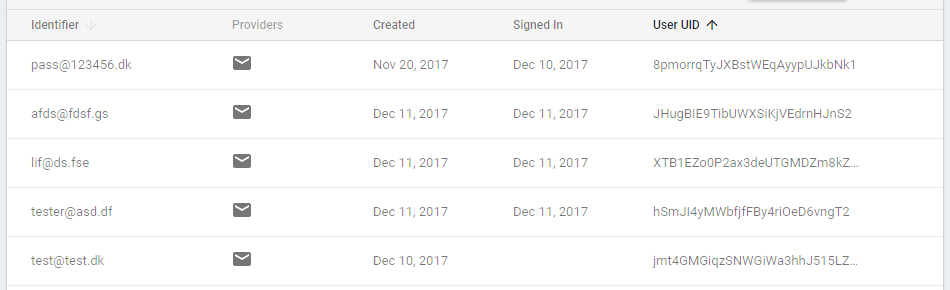
\includegraphics[height=5cm, width=15cm]{Design/Firebase/FirebaseAuth}
	\caption{Oversigt over authentication data i Firebase Console.}
	\label{fig:FirebaseAuthPNG}
\end{figure}
Denne indeholder en tabel, med en identifier som er brugerens e-mail. \\
Provider fortæller, hvordan brugeren har oprettet sig, som hænger sammen med created feltet, der fortæller, hvornår brugernen er oprettet. \\
Signed In fortæller, hvornår brugeren sidst er logget ind og det sidste felt er brugerens unikke id. \\
Her er også gemt et hashed password, men dette bliver ikke vist pga sikkerhed. \\

\clearpage

Figur \ref{fig:FirebaseDB} vises database strukturen i Firebase. 
\begin{figure}[H] % (alternativt [H])
	\centering
	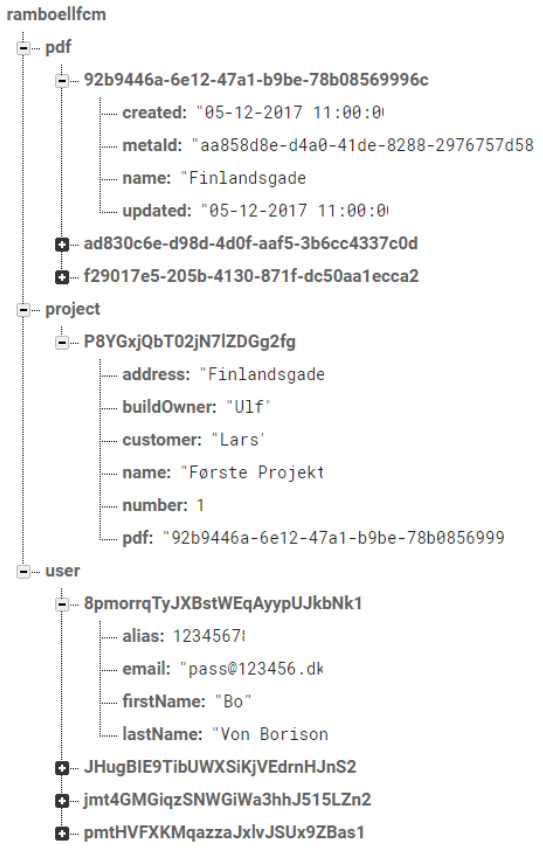
\includegraphics[height=12cm, width=10cm]{Design/Firebase/FirebaseDB}
	\caption{Oversigt strukturen i Firebase databasen}
	\label{fig:FirebaseDB}
\end{figure}
Databasen består af tre noder: \textbf{pdf}, \textbf{projekt} og \textbf{user}. \\
\textbf{pdf} noden indeholder alle PDF-tegninger i systemet, samt en reference til informationen omkring oprettede objekter på disse PDF filer. \\
Hver ny PDF, som bliver tilføjet i systemet, vil blive oprettet som en undernode i \textbf{pdf} noden. \\
\textbf{projekt} noden indeholder noder for hvert projekt som er oprettet. Disse undernoder indeholder alt det information som tilhører projekterne. \\
\textbf{user} noden indeholder information for brugere. Hver bruger oprettes som en ny undernode.

\clearpage